\documentclass[aspectratio=169,10pt,compress]{beamer}

\useoutertheme{split}
\useinnertheme{rounded}
\usecolortheme{whale}
\usecolortheme{orchid}
\setbeamertemplate{blocks}[rounded]
\setbeamertemplate{navigation symbols}{}
\setbeamertemplate{page number in head/foot}[totalframenumber]
% split footline shows "i / N" (frame number / total frames) on every frame

\usepackage[T1]{fontenc}
\usepackage{lmodern}
\usepackage{listings}
\usepackage{xcolor}
\usepackage{booktabs}
\usepackage{array}
\newcolumntype{L}[1]{>{\raggedright\arraybackslash}p{#1}}
\usepackage{tikz}
\usetikzlibrary{positioning,arrows.meta,calc}

\definecolor{codebg}{RGB}{245,245,245}
\definecolor{codecomment}{RGB}{110,110,110}
\definecolor{gitred}{RGB}{240,80,50}
\definecolor{gitblue}{RGB}{40,90,160}

\lstset{
  language=bash,
  basicstyle=\ttfamily\footnotesize,
  backgroundcolor=\color{codebg},
  commentstyle=\color{codecomment}\itshape,
  keywordstyle=\color{gitred}\bfseries,
  morekeywords={git},
  frame=single,
  rulecolor=\color{gray!40},
  columns=fullflexible,
  keepspaces=true,
  showstringspaces=false,
  breaklines=true,
  xleftmargin=4pt,
  xrightmargin=4pt,
  aboveskip=4pt,
  belowskip=4pt
}

\newcommand{\cmd}[1]{\texttt{\color{gitred}#1}}

\tikzset{
  commit/.style={circle, draw=gitblue, fill=gitblue!15, thick, minimum size=7mm,
                 inner sep=0pt, font=\scriptsize\ttfamily},
  newcommit/.style={commit, draw=gitred, fill=gitred!15},
  edge/.style={-{Stealth[length=2mm]}, thick, gray!70},
  lbl/.style={font=\scriptsize\bfseries, text=gitred}
}

\title{Git for Juniors}
\subtitle{Collaboration and Clean History}
\author[Bingol]{Haluk O. Bingol}

\institute[FCIS]{
    Faculty of Computer and Information Sciences\\
    Yeditepe University
}
\date{}

\begin{document}

% ~~~~~~~~~~~~~~~~~~~~~~~~~~~~~~~~~~~~~~ V
\begin{frame}[t,fragile]
  \titlepage
\end{frame}
% ~~~~~~~~~~~~~~~~~~~~~~~~~~~~~~~~~~~~~~ A

% ~~~~~~~~~~~~~~~~~~~~~~~~~~~~~~~~~~~~~~ V
\begin{frame}[t,fragile] \frametitle{Outline}
  \begin{columns}[T]
    \begin{column}{0.5\textwidth}
      \tableofcontents[sections={1-5}]
    \end{column}
    \begin{column}{0.5\textwidth}
      \tableofcontents[sections={6-11}]
    \end{column}
  \end{columns}
\end{frame}
% ~~~~~~~~~~~~~~~~~~~~~~~~~~~~~~~~~~~~~~ A

% ~~~~~~~~~~~~~~~~~~~~~~~~~~~~~~~~~~~~~~ V
\begin{frame}[t,fragile] \frametitle{Where we are}
  \textbf{You already know} (freshman and sophomore levels):
  \begin{itemize}
    \item commits, branches, merging, conflicts; the commit graph and \texttt{HEAD}
    \item \cmd{fetch} vs.\ \cmd{pull}, tracking branches, rejected pushes
    \item shared-repo teamwork: feature branches, pull requests, code review, issues
    \item basic \cmd{git stash} / \cmd{git stash pop}
  \end{itemize}

  \vspace{0.5em}
  \textbf{This lecture:} working like a professional
  \begin{itemize}
    \item contributing to projects you don't own, through forks
    \item keeping history clean and readable
    \item undoing mistakes with confidence
  \end{itemize}

  \vspace{0.5em}
  \begin{block}{Goal}
    Your pull requests should be easy to review and your history easy to read.
  \end{block}
\end{frame}
% ~~~~~~~~~~~~~~~~~~~~~~~~~~~~~~~~~~~~~~ A

% ~~~~~~~~~~~~~~~~~~~~~~~~~~~~~~~~~~~~~~ V
\section[Forks]{Forks and Upstream}
% ~~~~~~~~~~~~~~~~~~~~~~~~~~~~~~~~~~~~~~ A

% ~~~~~~~~~~~~~~~~~~~~~~~~~~~~~~~~~~~~~~ V
\begin{frame}[t,fragile] \frametitle{Fork vs.\ clone}
  \begin{center}
  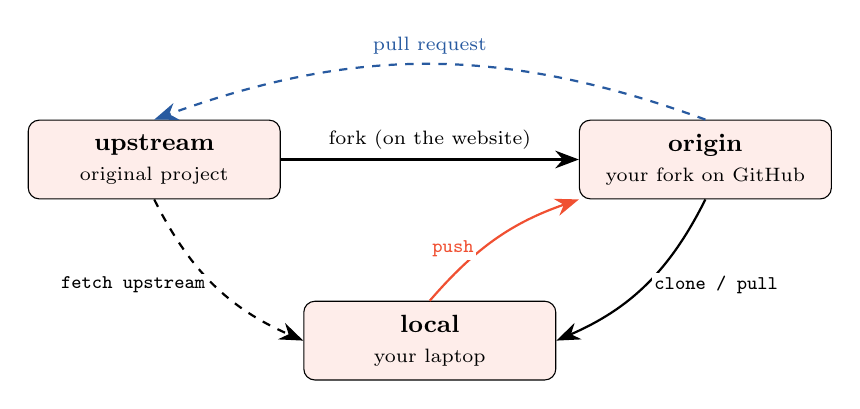
\begin{tikzpicture}[
      box/.style={draw, rounded corners, fill=gitred!10, minimum width=3.2cm,
                  minimum height=1cm, align=center, font=\small},
      arr/.style={-{Stealth[length=3mm]}, thick},
      t/.style={font=\scriptsize\ttfamily, fill=white, inner sep=1pt}]
    \node[box] (up) at (0,0) {\textbf{upstream}\\ \scriptsize original project};
    \node[box] (or) at (7,0) {\textbf{origin}\\ \scriptsize your fork on GitHub};
    \node[box] (loc) at (3.5,-2.3) {\textbf{local}\\ \scriptsize your laptop};
    \draw[arr] (up.east) -- node[above, font=\scriptsize]{fork (on the website)} (or.west);
    \draw[arr, dashed, gitblue] (or.north) to[bend right=20]
          node[above, font=\scriptsize]{pull request} (up.north);
    \draw[arr] (or.south) to[bend left=20] node[t, right=2pt]{clone / pull} (loc.east);
    \draw[arr, gitred] (loc.north) to[bend left=15] node[t, pos=0.4, left=2pt]{push} (or.south west);
    \draw[arr, dashed] (up.south) to[bend right=20] node[t, left=2pt]{fetch upstream} (loc.west);
  \end{tikzpicture}
  \end{center}

  \begin{itemize}
    \item \textbf{Clone:} a local copy. Use it when you have write access.
    \item \textbf{Fork:} your own server-side copy. Use it when you don't have write access (open source).
  \end{itemize}
\end{frame}
% ~~~~~~~~~~~~~~~~~~~~~~~~~~~~~~~~~~~~~~ A

% ~~~~~~~~~~~~~~~~~~~~~~~~~~~~~~~~~~~~~~ V
\begin{frame}[t,fragile] \frametitle{Keeping a fork in sync}
\begin{lstlisting}
git clone https://github.com/you/project.git
cd project
git remote add upstream https://github.com/owner/project.git
git remote -v                     # origin = your fork, upstream = original

# later: bring in new work from the original project
git fetch upstream
git switch main
git merge upstream/main           # or: git rebase upstream/main
git push origin main              # update your fork too
\end{lstlisting}

  \begin{block}{Rule of thumb}
    Never commit directly on \texttt{main} in a fork. Keep it a clean mirror of
    \texttt{upstream/main} and do all work on feature branches.
  \end{block}
\end{frame}
% ~~~~~~~~~~~~~~~~~~~~~~~~~~~~~~~~~~~~~~ A

% ~~~~~~~~~~~~~~~~~~~~~~~~~~~~~~~~~~~~~~ V
\begin{frame}[t,fragile] \frametitle{Pull requests from a fork}
  You already know PRs inside a shared repo. From a fork, three things change:
  \begin{enumerate}
    \item The PR goes \emph{across repositories}:
          \texttt{you/project:fix-timeout} $\rightarrow$ \texttt{owner/project:main}
    \item You can't push to \texttt{upstream}. Keep your branch current by rebasing it on
          \texttt{upstream/main}, then \cmd{git push --force-with-lease} to your fork
    \item Maintainers you don't know will review it, often asking you to squash or reword commits
  \end{enumerate}

  \vspace{0.3em}
  \small
  \begin{tabular}{@{}L{0.26\textwidth}L{0.66\textwidth}@{}}
    \toprule
    \textbf{Maintainer merges with} & \textbf{Result on \texttt{main}} \\
    \midrule
    Merge commit & all your commits, plus a merge commit \\
    Squash and merge & your whole PR becomes one commit \\
    Rebase and merge & your commits replayed on top, no merge commit \\
    \bottomrule
  \end{tabular}

  \normalsize
  \vspace{0.3em}
  That is why the rest of this lecture is about rebasing and clean history.
\end{frame}
% ~~~~~~~~~~~~~~~~~~~~~~~~~~~~~~~~~~~~~~ A

% ~~~~~~~~~~~~~~~~~~~~~~~~~~~~~~~~~~~~~~ V
\section[Strategies]{Branching Strategies}
% ~~~~~~~~~~~~~~~~~~~~~~~~~~~~~~~~~~~~~~ A

% ~~~~~~~~~~~~~~~~~~~~~~~~~~~~~~~~~~~~~~ V
\begin{frame}[t,fragile] \frametitle{Branching strategies}
  \small
  \begin{tabular}{@{}L{0.2\textwidth}L{0.44\textwidth}L{0.3\textwidth}@{}}
    \toprule
    \textbf{Strategy} & \textbf{How it works} & \textbf{Good for} \\
    \midrule
    Feature branching & One branch per feature or fix, merged into \texttt{main} via PR
      & Most student and team projects \\[4pt]
    Trunk-based & Everyone merges tiny changes into \texttt{main} daily; unfinished work hidden behind feature flags
      & Teams with strong CI and tests \\[4pt]
    GitFlow & Long-lived \texttt{develop} and \texttt{main}, plus \texttt{feature/}, \texttt{release/}, \texttt{hotfix/}
      & Versioned products with scheduled releases \\
    \bottomrule
  \end{tabular}

  \vspace{1em}
  \begin{block}{The lesson that matters most}
    Keep branches \textbf{short-lived}. The longer a branch lives, the harder it is to merge.
  \end{block}
\end{frame}
% ~~~~~~~~~~~~~~~~~~~~~~~~~~~~~~~~~~~~~~ A

% ~~~~~~~~~~~~~~~~~~~~~~~~~~~~~~~~~~~~~~ V
\section[Rebase]{Rebase vs.\ Merge}
% ~~~~~~~~~~~~~~~~~~~~~~~~~~~~~~~~~~~~~~ A

% ~~~~~~~~~~~~~~~~~~~~~~~~~~~~~~~~~~~~~~ V
\begin{frame}[t,fragile] \frametitle{Two ways to combine work}
  \begin{columns}[T]
    \begin{column}{0.5\textwidth}
      \centering\textbf{\cmd{git merge feature}}\\[4pt]
      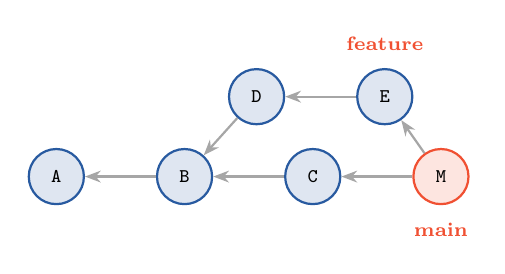
\begin{tikzpicture}[node distance=9mm]
        \node[commit] (a) {A};
        \node[commit, right=of a] (b) {B};
        \node[commit, right=of b] (c) {C};
        \node[commit, above right=5mm and 4mm of b] (d) {D};
        \node[commit, right=of d] (e) {E};
        \node[newcommit, right=of c] (m) {M};
        \draw[edge] (b) -- (a); \draw[edge] (c) -- (b);
        \draw[edge] (d) -- (b); \draw[edge] (e) -- (d);
        \draw[edge] (m) -- (c); \draw[edge] (m) -- (e);
        \node[lbl, below=1mm of m] {main};
        \node[lbl, above=1mm of e] {feature};
      \end{tikzpicture}\\[4pt]
      \small
      \begin{itemize}
        \item Keeps true history
        \item Adds a merge commit \texttt{M}
        \item Safe on shared branches
      \end{itemize}
    \end{column}
    \begin{column}{0.5\textwidth}
      \centering\textbf{\cmd{git rebase main}} (on feature)\\[4pt]
      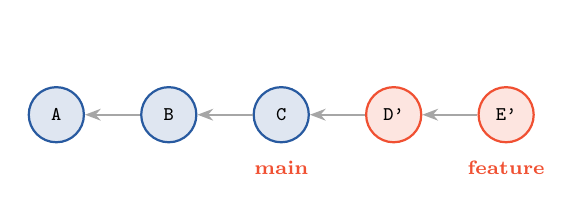
\begin{tikzpicture}[node distance=7mm]
        \node[commit] (a) {A};
        \node[commit, right=of a] (b) {B};
        \node[commit, right=of b] (c) {C};
        \node[newcommit, right=of c] (d) {D'};
        \node[newcommit, right=of d] (e) {E'};
        \draw[edge] (b) -- (a); \draw[edge] (c) -- (b);
        \draw[edge] (d) -- (c); \draw[edge] (e) -- (d);
        \node[lbl, below=1mm of c] {main};
        \node[lbl, below=1mm of e] {feature};
        \node[above=5mm of b] {};
      \end{tikzpicture}\\[4pt]
      \small
      \begin{itemize}
        \item Linear, easy-to-read history
        \item Creates \emph{new} commits \texttt{D'}, \texttt{E'}
        \item Rewrites history
      \end{itemize}
    \end{column}
  \end{columns}
\end{frame}
% ~~~~~~~~~~~~~~~~~~~~~~~~~~~~~~~~~~~~~~ A

% ~~~~~~~~~~~~~~~~~~~~~~~~~~~~~~~~~~~~~~ V
\begin{frame}[t,fragile] \frametitle{Rebasing in practice}
\begin{lstlisting}
git switch feature
git fetch origin
git rebase origin/main            # replay my commits on top of latest main
# conflict? fix the file, then:
git add <file>
git rebase --continue             # or: git rebase --abort to give up

git push --force-with-lease       # branch was rewritten, so push must force
\end{lstlisting}

  \begin{columns}[T]
    \begin{column}{0.48\textwidth}
      \begin{alertblock}{The golden rule}
        Never rebase commits that others have already pulled.
        Rebase \emph{your own} unshared branches only.
      \end{alertblock}
    \end{column}
    \begin{column}{0.48\textwidth}
      \begin{block}{Tip}
        \cmd{git pull --rebase} avoids noisy ``Merge branch main'' commits.
        Make it the default: \cmd{git config --global pull.rebase true}
      \end{block}
    \end{column}
  \end{columns}
\end{frame}
% ~~~~~~~~~~~~~~~~~~~~~~~~~~~~~~~~~~~~~~ A

% ~~~~~~~~~~~~~~~~~~~~~~~~~~~~~~~~~~~~~~ V
\section[Rebase -i]{Interactive Rebase}
% ~~~~~~~~~~~~~~~~~~~~~~~~~~~~~~~~~~~~~~ A

% ~~~~~~~~~~~~~~~~~~~~~~~~~~~~~~~~~~~~~~ V
\begin{frame}[t,fragile] \frametitle{Cleaning up with \texttt{git rebase -i}}
  Before opening a PR, turn messy work-in-progress into a clean story:
\begin{lstlisting}
git rebase -i main                # edit all commits since main
\end{lstlisting}
  Git opens an editor with a ``todo list'':
\begin{lstlisting}[language={}]
pick   a1b2c3d Add login form
squash e4f5a6b wip
squash 9c8d7e6 fix typo
reword 1f2e3d4 validation
drop   5a6b7c8 debug prints
\end{lstlisting}
  \small
  \begin{tabular}{@{}ll@{\hspace{2em}}ll@{}}
    \texttt{pick}   & keep as is           & \texttt{squash} & merge into previous, combine messages \\
    \texttt{reword} & change the message   & \texttt{fixup}  & merge into previous, discard message \\
    \texttt{edit}   & stop to amend/split  & \texttt{drop}   & delete the commit \\
  \end{tabular}
\end{frame}
% ~~~~~~~~~~~~~~~~~~~~~~~~~~~~~~~~~~~~~~ A

% ~~~~~~~~~~~~~~~~~~~~~~~~~~~~~~~~~~~~~~ V
\begin{frame}[t,fragile] \frametitle{Fixup commits and autosquash}
  You spot a bug in a commit you made three commits ago. Instead of a
  ``fix typo'' commit at the end:

\begin{lstlisting}
git log --oneline
#   7d1e2f3 Add tests
#   4c5b6a7 Add password check
#   a1b2c3d Add login form        <- the bug is here

# fix the file, then:
git add login.py
git commit --fixup a1b2c3d        # creates "fixup! Add login form"

git rebase -i --autosquash main   # moves the fix next to its target
\end{lstlisting}

  \begin{block}{Result}
    The fix is folded into \texttt{a1b2c3d}, as if you had written it correctly the first time.
  \end{block}
\end{frame}
% ~~~~~~~~~~~~~~~~~~~~~~~~~~~~~~~~~~~~~~ A

% ~~~~~~~~~~~~~~~~~~~~~~~~~~~~~~~~~~~~~~ V
\section[Stash]{Stashing and Partial Staging}
% ~~~~~~~~~~~~~~~~~~~~~~~~~~~~~~~~~~~~~~ A

% ~~~~~~~~~~~~~~~~~~~~~~~~~~~~~~~~~~~~~~ V
\begin{frame}[t,fragile] \frametitle{Stash beyond \texttt{pop}}
  You know \cmd{git stash} and \cmd{git stash pop}. The rest of the toolbox:
\begin{lstlisting}
git stash push -m "half-done search"   # name it so you can find it later
git stash push -u                      # include untracked (new) files too
git stash push -- src/search.py        # stash only some files

git stash list                         # stash@{0}, stash@{1}, ...
git stash show -p stash@{1}            # what's inside?
git stash apply stash@{1}              # apply but keep it in the list
git stash drop stash@{1}               # delete it
git stash branch search-wip stash@{1}  # new branch from where it was made
\end{lstlisting}

  \begin{alertblock}{When \texttt{pop} conflicts}
    If the stash doesn't apply cleanly, Git keeps it in the list. Resolve the conflict,
    then \cmd{git stash drop}. \cmd{git stash branch} avoids the conflict entirely.
  \end{alertblock}
\end{frame}
% ~~~~~~~~~~~~~~~~~~~~~~~~~~~~~~~~~~~~~~ A

% ~~~~~~~~~~~~~~~~~~~~~~~~~~~~~~~~~~~~~~ V
\begin{frame}[t,fragile] \frametitle{Partial staging with \texttt{git add -p}}
  One file contains two unrelated changes. Commit them separately:
\begin{lstlisting}
git add -p parser.py
\end{lstlisting}
  Git shows each change (``hunk'') and asks what to do:
\begin{lstlisting}[language={}]
@@ -12,6 +12,7 @@ def parse(line):
-    tokens = line.split(",")
+    tokens = line.strip().split(",")
Stage this hunk [y,n,q,a,d,s,e,?]?
\end{lstlisting}
  \small
  \begin{tabular}{@{}ll@{\hspace{2em}}ll@{}}
    \texttt{y} & stage this hunk      & \texttt{s} & split into smaller hunks \\
    \texttt{n} & skip this hunk       & \texttt{e} & edit the hunk by hand \\
    \texttt{q} & quit                 & \texttt{?} & help \\
  \end{tabular}

  \vspace{0.5em}
  \normalsize
  Then \cmd{git diff --staged} to review before \cmd{git commit}.
\end{frame}
% ~~~~~~~~~~~~~~~~~~~~~~~~~~~~~~~~~~~~~~ A

% ~~~~~~~~~~~~~~~~~~~~~~~~~~~~~~~~~~~~~~ V
\section[Undo]{Undoing Things}
% ~~~~~~~~~~~~~~~~~~~~~~~~~~~~~~~~~~~~~~ A

% ~~~~~~~~~~~~~~~~~~~~~~~~~~~~~~~~~~~~~~ V
\begin{frame}[t,fragile] \frametitle{The three modes of \texttt{git reset}}
  \cmd{git reset <commit>} moves the current branch to \texttt{<commit>}.
  The mode decides what happens to your changes:

  \vspace{0.5em}
  \small
  \begin{tabular}{@{}lccc@{}}
    \toprule
    & \textbf{Branch (HEAD)} & \textbf{Staging area} & \textbf{Working files} \\
    \midrule
    \cmd{--soft}  & moved & kept & kept \\
    \cmd{--mixed} (default) & moved & reset & kept \\
    \cmd{--hard}  & moved & reset & \textcolor{red}{\textbf{reset (changes lost!)}} \\
    \bottomrule
  \end{tabular}

  \vspace{0.5em}
\begin{lstlisting}
git reset --soft HEAD~3     # "uncommit" last 3 commits, keep them staged
git reset HEAD~1            # uncommit and unstage, keep the edits
git reset --hard origin/main  # throw everything away, match the remote
\end{lstlisting}
\end{frame}
% ~~~~~~~~~~~~~~~~~~~~~~~~~~~~~~~~~~~~~~ A

% ~~~~~~~~~~~~~~~~~~~~~~~~~~~~~~~~~~~~~~ V
\begin{frame}[t,fragile] \frametitle{Choosing the right undo}
  \small
  \begin{tabular}{@{}L{0.37\textwidth}L{0.4\textwidth}L{0.18\textwidth}@{}}
    \toprule
    \textbf{Situation} & \textbf{Command} & \textbf{Rewrites history?} \\
    \midrule
    Discard edits to a file & \cmd{git restore <file>} & no \\
    Unstage a file & \cmd{git restore --staged <file>} & no \\
    Fix the last commit & \cmd{git commit --amend} & yes \\
    Uncommit local, unpushed work & \cmd{git reset} & yes \\
    Undo a commit already pushed & \cmd{git revert <sha>} & \textbf{no} \\
    Restore one file from an old commit & \cmd{git restore -s <sha> <file>} & no \\
    \bottomrule
  \end{tabular}

  \vspace{1em}
  \begin{alertblock}{Pushed = public}
    Once commits are pushed and shared, use \cmd{revert}, not \cmd{reset}.
    Revert adds a new commit that cancels the old one, so nobody else's history breaks.
  \end{alertblock}
\end{frame}
% ~~~~~~~~~~~~~~~~~~~~~~~~~~~~~~~~~~~~~~ A

% ~~~~~~~~~~~~~~~~~~~~~~~~~~~~~~~~~~~~~~ V
\section[Reflog]{The Reflog}
% ~~~~~~~~~~~~~~~~~~~~~~~~~~~~~~~~~~~~~~ A

% ~~~~~~~~~~~~~~~~~~~~~~~~~~~~~~~~~~~~~~ V
\begin{frame}[t,fragile] \frametitle{The reflog: Git's safety net}
  Oops: \cmd{git reset --hard HEAD\textasciitilde3} deleted three commits. Or did it?

\begin{lstlisting}
git reflog
#  3f4e5d6 HEAD@{0}: reset: moving to HEAD~3
#  9a8b7c6 HEAD@{1}: commit: Add export button
#  2d3c4b5 HEAD@{2}: commit: Add CSV writer
#  7e6f5a4 HEAD@{3}: commit: Add data model

git reset --hard 9a8b7c6          # go back to before the mistake
# or, more cautiously:
git branch rescue 9a8b7c6         # save them on a new branch
\end{lstlisting}

  \begin{block}{Why it works}
    The reflog records every place \texttt{HEAD} has pointed, locally, for about 90 days.
    Committed work is almost never truly lost. \textbf{Uncommitted} work is.
  \end{block}
\end{frame}
% ~~~~~~~~~~~~~~~~~~~~~~~~~~~~~~~~~~~~~~ A

% ~~~~~~~~~~~~~~~~~~~~~~~~~~~~~~~~~~~~~~ V
\section[History]{Inspecting History}
% ~~~~~~~~~~~~~~~~~~~~~~~~~~~~~~~~~~~~~~ A

% ~~~~~~~~~~~~~~~~~~~~~~~~~~~~~~~~~~~~~~ V
\begin{frame}[t,fragile] \frametitle{Reading history like a detective}
\begin{lstlisting}
git log --oneline --graph --all     # the whole branch structure
git log --author="Ayse" --since="2 weeks ago"
git log -p -- src/parser.py         # every change to one file
git log -S "calculate_gpa"          # commits that added/removed this text

git show a1b2c3d                    # one commit in full
git blame -L 40,60 src/parser.py    # who last changed lines 40-60?

git diff main..feature              # difference between two branch tips
git diff main...feature             # only what feature added since it branched
\end{lstlisting}

  \begin{block}{Tip}
    Make an alias: \cmd{git config --global alias.lg "log --oneline --graph --all"},
    then just type \cmd{git lg}.
  \end{block}
\end{frame}
% ~~~~~~~~~~~~~~~~~~~~~~~~~~~~~~~~~~~~~~ A

% ~~~~~~~~~~~~~~~~~~~~~~~~~~~~~~~~~~~~~~ V
\section[Tags]{Tags and Releases}
% ~~~~~~~~~~~~~~~~~~~~~~~~~~~~~~~~~~~~~~ A

% ~~~~~~~~~~~~~~~~~~~~~~~~~~~~~~~~~~~~~~ V
\begin{frame}[t,fragile] \frametitle{Tags and semantic versioning}
  \begin{columns}[T]
    \begin{column}{0.55\textwidth}
\begin{lstlisting}
# annotated tag: author, date, message
git tag -a v1.2.0 -m "Release 1.2.0"
# lightweight tag: just a name
git tag v1.2.0-rc1

git tag                 # list tags
git show v1.2.0
git push origin v1.2.0  # tags aren't
                        # pushed by default
git push origin --tags
\end{lstlisting}
    \end{column}
    \begin{column}{0.42\textwidth}
      \textbf{Semantic versioning}\\[2pt]
      \texttt{MAJOR.MINOR.PATCH}
      \begin{itemize}\small
        \item \textbf{MAJOR:} breaking change
        \item \textbf{MINOR:} new feature, compatible
        \item \textbf{PATCH:} bug fix only
      \end{itemize}
      \vspace{0.3em}
      \small Example: \texttt{2.4.1} $\rightarrow$ \texttt{2.5.0} adds a feature;
      \texttt{3.0.0} breaks the API.
    \end{column}
  \end{columns}

  \begin{block}{Releases}
    On GitHub, a \emph{Release} is a tag plus release notes and downloadable files.
    Use annotated tags for releases.
  \end{block}
\end{frame}
% ~~~~~~~~~~~~~~~~~~~~~~~~~~~~~~~~~~~~~~ A

% ~~~~~~~~~~~~~~~~~~~~~~~~~~~~~~~~~~~~~~ V
\section[Commits]{Commit Conventions}
% ~~~~~~~~~~~~~~~~~~~~~~~~~~~~~~~~~~~~~~ A

% ~~~~~~~~~~~~~~~~~~~~~~~~~~~~~~~~~~~~~~ V
\begin{frame}[t,fragile] \frametitle{Writing commits for other people}
  \begin{columns}[T]
    \begin{column}{0.5\textwidth}
      \textbf{Anatomy of a good message}
\begin{lstlisting}[language={}]
Fix crash when grade list is empty

average() divided by len(grades)
without checking for zero. Return
None for an empty list and show
"no grades yet" in the UI.

Closes #42
\end{lstlisting}
      \small
      \begin{itemize}
        \item Subject: imperative, $\le$ 50 chars
        \item Blank line, then \emph{why}
      \end{itemize}
    \end{column}
    \begin{column}{0.47\textwidth}
      \textbf{Conventional Commits}
\begin{lstlisting}[language={}]
feat: add CSV export
fix: handle empty grade list
docs: explain setup on Windows
refactor: split parser module
test: cover leap years
feat!: drop Python 3.8 support
\end{lstlisting}
      \small
      Tools can generate changelogs and version bumps from these prefixes.
    \end{column}
  \end{columns}

  \begin{block}{Atomic commits}
    One logical change per commit: it builds, tests pass, and it can be reverted on its own.
  \end{block}
\end{frame}
% ~~~~~~~~~~~~~~~~~~~~~~~~~~~~~~~~~~~~~~ A

% ~~~~~~~~~~~~~~~~~~~~~~~~~~~~~~~~~~~~~~ V
\section[Labs]{Labs and Summary}
% ~~~~~~~~~~~~~~~~~~~~~~~~~~~~~~~~~~~~~~ A

% ~~~~~~~~~~~~~~~~~~~~~~~~~~~~~~~~~~~~~~ V
\begin{frame}[t,fragile] \frametitle{Lab exercises}
  \begin{enumerate}
    \item \textbf{Fork and PR:} fork the course repo, add your name to
          \texttt{STUDENTS.md} on a branch, and open a pull request.
    \item \textbf{Sync:} after the instructor merges others' PRs, sync your fork
          with \texttt{upstream} and resolve any conflict.
    \item \textbf{Clean up:} make 6 messy commits (``wip'', ``typo'', ...),
          then use \cmd{rebase -i} to turn them into 2 clean ones.
    \item \textbf{Fixup:} fix a bug in an older commit using
          \cmd{--fixup} and \cmd{--autosquash}.
    \item \textbf{Disaster recovery:} run \cmd{git reset --hard HEAD\textasciitilde5},
          then recover every commit using the reflog.
    \item \textbf{Detective:} in a given repo, find who introduced the function
          \texttt{legacy\_import} and when, using \cmd{log -S} and \cmd{blame}.
  \end{enumerate}
\end{frame}
% ~~~~~~~~~~~~~~~~~~~~~~~~~~~~~~~~~~~~~~ A

% ~~~~~~~~~~~~~~~~~~~~~~~~~~~~~~~~~~~~~~ V
\begin{frame}[t,fragile] \frametitle{Cheat sheet}
  \begin{columns}[T]
    \begin{column}{0.49\textwidth}
\begin{lstlisting}
git remote add upstream <url>
git fetch upstream
git rebase origin/main
git rebase -i main
git commit --fixup <sha>
git rebase -i --autosquash main
git push --force-with-lease
git pull --rebase
\end{lstlisting}
    \end{column}
    \begin{column}{0.49\textwidth}
\begin{lstlisting}
git stash list / apply / -u
git add -p
git reset --soft|--mixed|--hard
git revert <sha>
git reflog
git log --oneline --graph --all
git log -S "text" / git blame
git tag -a v1.0.0 -m "msg"
\end{lstlisting}
    \end{column}
  \end{columns}

  \vspace{1em}
  \begin{center}
    {\Large \textbf{Questions?}}
  \end{center}
\end{frame}
% ~~~~~~~~~~~~~~~~~~~~~~~~~~~~~~~~~~~~~~ A

\end{document}
